% -*-coding: utf-8 -*-

\defaultfont
\appendix

%%%%%%%%%%%%%%%%%%%%%%%%%%%%%%%%%%%%%%%%%%%%%%%%%%%%%%%%%
\BiAppChapter{深度学习——人工智能研究的新前沿}{AppendixB}%
\BiSection{导言}
x模仿人类的大脑表示信息的高效性和稳健性一直是近几十年来人工智能研究的一个核心挑战。一天中的每秒,人都在接收无数感官数据,并能在某种程度上通过允许在未来能以简洁方式使用的方式捕获数据的重要方面,通过允许在未来能以简洁方式使用的方式。50年多前,提出动态规划理论和开创最优控制领域的 Richard Bellman 断言数据的高维性是在许多科学和工程应用中的基本障碍。主要的困难是学习复杂性随着数据的维数线性增加呈指数增长,尤其在模式分类应用中。他把这个现象叫做维数灾难。克服“灾难”的主流方法是预先处理数据,通过这种方式将它的维数减少到分类器可以有效进行处理的维度。这个维数降低方案通常被称为特征提取。结果表明,许多模式识别系统背后的智能可转化为工程化的特征提取过程,这有时是很有挑战性的,且高度依赖于应用。此外,如果提取的特征是不完整的或错误的,会在本质上限制分类性能。

最近的神经科学的深入研究结果揭示了在哺乳动物大脑对信息表示的管理原则,引出了设计代表信息的系统的新想法。一个重要的发现是,被认为与许多的认知能力有关的新皮层,并没有明确预处理感知信号,而是允许它们通过一个复杂的分层传播的模块,随着时间的推移,基于它们显示出的规律学习表示观察结果。这一发现促使子研究领域深度学习的出现,它侧重于用于与大脑皮层有相似特征的信息表达的计算模型。

除了现实生活中的数据的空间维度,时间分量也起着关键的作用。图案的观测序列往往传达一个意思给观察者,然而,该序列的独立片段将很难孤立地解读。含义往往是从在时间上最近收到事件或观察上推断出的。为达此目的,对观测物体的时间部分进行建模在有效的信息表示中的起着关键作用。基于观测的规律捕获时空相关性,被视为深度学习系统的一个基本目的。

假设健壮的深度学习已经被实现,它可能在一大组观察结果上训练出这样一个分层网络,然后从这个网络提取信号到一个相对简单的分类器以达到健壮的辨别图片的目的。稳健在这里指的是对各种各样的变换和扭曲,包括噪声,缩放,旋转,不同的光照等条件下,位移等表现出来的分类不变性。

本文提供了在过去十年的主流深度学习的方法和研究方向的概述。必须强调的是每种方法都有优点和缺点,这取决于它被应用到的应用程序和环境。因此,本文提出了对深度学习领域当前状态的总结和一些观点以推测到它可能如何演变。首先关注卷积神经网络(CNN)和深度置信网络(DBN)(及其各自的变化),因为它们都在深度学习领域建立的很好,并在今后的工作中大有希望。第二节介绍了CNN,并随后在第三节详细介绍了DBN。为更好的进一步深入了解这些技术的基础,读者可以参考文献《Learning deep architectures for AI》。第四节包含了近期提出的其他的深度架构。第五节包含一个简短的说明,这个说明关于这个研究是如何已经影响政府和行业活动的。结论提供了对深层次架构的潜在影响的看法,以及仍然存在需要回答的关键问题。

\BiSection{卷积神经网络}
xCNN为针对二维数据例如图像和视频而特别设计的多层神经网络。CNN受早期的时迟神经网络(TDNN)影响。TDNN要求通过在时间维度共享权数降低学习计算需求,且旨在对语音和时间序列进行处理。CNN是第一个真正成功的深度学习的方法,其中一个层级的许多层被成功地训练出一种健壮的方式。CNN是拓扑结构或架构的一种选择,它充分利用空间和时间的关系,以减少必须学会的参数的数量,从而在一般的前馈反向传播训练中有了提升。CNN作为出于最小数据预处理要求的深度学习框被提出。在CNN中,所述图像(称为一个局部感知域)的一小部分被当作输入该分层结构的最低层。信息通常通过网络的不同层传播,由此在每一层都会应用数字滤波以获得所观察到的数据的显着特征。该方法提供一定程度的对平移、比例和旋转的不变性,同时局部感知域允许神经元或处理单元连接到基本特征如面向边或角。

其中一个关于这个专题的重要论文《Gradient-based learning applied to document recognition》介绍CNN对笔迹分析问题的应用。本质上,该输入图像和一组N小的过滤器进行卷积运算,其系数被训练,或使用一些标准预先确定。因此,网络的第一(或最低)层由“特征图”组成,这是卷积过程的结果,且具有正偏差以及可能的对特征的压缩或正常化。此初始阶段之后是降采样(通常为2x2平均运算),该阶段进一步降低维数,并提供一定的对空间变化的鲁棒性(见图2)。二次取样特征图然后接收加权和训练的偏差,最终通过激活功能传播。这方面有一些变体存在,为尽可能少每层一个图或多个图的总和。

当加权小时,激活函数是近似线性的,其结果是所述图像的模糊; 其他加权可导致激活的输出类似于一个AND或OR功能。这些输出形成一个新的特征图,然后新的特征图通过另一个卷积序列,子采样和激活功能,如图3所示。该过程可以重复任意次数。应当指出的是,随后的层可以结合一个或多个先前的层; 例如,在《Gradient-based learning applied to document recognition》中,最初六个特征图相结合以形成在后继层的16特征图。如在《“How the brain might work: A hierarchical and temporal model for learning and recognition”》中描述的,CNN通过被称为“特征池”的方法创建他们对对象的翻译不变(如图3中S层所示)。然而,特征池是网络组织者手工制作的,没有经过系统的培训或学习; 在CNN中,该池通过在学习过程中由参数进行“调整”,但基本的机构(例如,输入到S层的组合)由网络设计者设置。最后,在过程的最后阶段,激活输出被转发到产生该系统的最终输出的常规的前馈神经网络。

在CNN中,层次和空间信息之间的亲密关系使得它们非常适合于图像处理和理解,他们通常在从图像中自主提取显着特征方面表现良好。在某些情况下,Gabor滤波器已被用来作为初始的预处理步骤以模拟到人类对视觉激发的视觉响应。在最近的工作中,研究人员已应用CNN到各种机器学习的问题上,包括人脸检测,文档分析,和语音检测。CNN最近用时间一致的对象训练以在视频中能达到帧到帧的一致性,尽管这目标不必是特定于CNN的。

\BiSection{深度置信网络}
xDBN,在最初在《A fast learning algorithm for deep belief nets》中提出,与传统的神经网络的判别性质形成对比概率生成模型。生成模型提供观察数据和标签的联合概率分布, P(Observation|Label)和P(Label|Observation)的估计更容易,而判别模型受限于后者,P(Label|Observation)。DBN解决所遇到的问题时,采用传统的反向传播至深层次的神经网络,即:(1)用于训练的大幅标记的数据集的必要性,(2)慢的学习次数(即收敛),(3)导致不良局部最优的不足的参数选择技术。

DBN由几层波尔兹曼机构成,是一种神经网络(见图1)。这些网络被“限制”在层之间形成的(在层内单元未连接)一个可见层和一个隐藏层。隐藏的单元被训练用来捕捉那些在可见的单元观察到的高阶数据的相关性。最初,除了形成一个相联存贮器的顶部的两个层, DBN仅由直接自上而下生成的权重连接。RBM作为结构单元在更传统的和深层S形置信网络很有吸引力,因为它们易于学习这些连接权。为了获得生成的权重,在初始预训练以无监督的贪婪的层-层的方式进行,通过Hinton称作对比离差的东西使能。在这个训练阶段,一个矢量v被呈现给可见单元并转发值到隐藏的单位。朝着相反的,在可见单元输入然后随机的在重建原始输入的尝试中找到。最后,这些新的可见神经元的激活被转发,使得重建隐藏单元的激活的步骤,h,可以实现。执行这些来回步骤被称为Gibbs抽样的方法,在隐藏激活和可见输入的相关的差异形成了权值更新的基础。训练时间显著降低,因为它可以证明,对于近似最大似然学习只有一个步骤是必要的。添加到网络中的每个层都改善了训练数据的对数概率,我们可以认为对数概率是增加真正代表性功率的。这项有意义的扩展,与未标记数据的利用相结合,在任何深度学习应用中都是重要组成部分。

在顶部两层,权重被连接在一起,以使得下层的输出为顶层联系其存储器内容提供参考线索或连结。我们经常遇到的问题中,判别性能的最终焦点,如在分类任务中。DBN可以通过反向传播利用标记的数据在预训练之后进行微调以提高判别性能。此时,一组标签被附着到顶层(扩大相联存储器),以澄清网络中类别的边界,通过这样,一组新的自下而上,识别权重被学习。《Reducing the dimensionality of data with neural networks》已经表明,这种网络经常表现的比那些训练有素只有反向传播的要好。这可以通过以下事实直观的解释。DBN相对于传统的前馈神经网络来说,反向传播时,才需要在权重(参数)空间中进行局部搜索,加快了训练和收敛时间。

运用DBN到MNIST手写字符识别任务时获得的性能结果表明显著改善了前馈网络。引入DBN之后不久,《Greedy layer-wise training of deep networks》中更透彻的分析固化了它们是无监督的任务以及连续值的输入的特点。《Unsupervised learning of invariant feature hierarchies with applications to object recognition》与《An empirical evaluation of deep architectures on problems with many factors of variation》进一步的测试表明DBN(以及其它深架构)面对变化不停增长的问题的恢复力。

通过引入卷积深层置信网络(CDBN)的概念,DBN的灵活性最近扩大。DBN不固有地嵌入关于输入的图像的二维结构的信息,即输入是简单矢量格式的图像矩阵。与此相反,CDBN利用相邻像素的空间关系,引入被称作卷积RBM来提供一种具有高尺寸图像缩放以及平移不变生成模型的空间关系。DBN目前没有明确处理学习观测量之间的时间关系,虽然最近有工作在堆叠颞RBM 或这些的概括,被称为颞卷积机[23],用于学习的序列。这样的序列学习者被应用到音频信号处理问题上,从而DBN最近已经取得了进展 ,提供了一个途径令人振奋的未来的研究方向。

用于DBN和CNN的静态图像测试中最常见的是手写数字的MNIST数据库和加州理工学院-101数据库的各种对象(属于101类)。每个体系结构的分类错误率可以在[19] [20] [21]中找到。[27]提供了应用到MNIST数据库的各种机器学习技术的全面且最新的性能比较。

最近有关DBN的作品包括使用堆叠自动编码器代替传统DBN下的RBM[17] [18] [21]。这种努力产生的深多层神经网络架构可以用和DBN相同的原则训练,但在对层的参数更不严格。不像DBN,自动编码器使用的是输入样本空间不能由结构进行采样的判别模型,使得它更难以解释在其内部什么网络被捕获。然而,[21]已经表明,去噪的自动编码器,在训练期间会随机失效,和传统DBN相比可能被堆叠以产生泛化性能(且在某些情况下,更好的是DBN)。对于单个去噪自动编码器训练过程对应于用于生成模型如RBMS的目标。

\BiSection{最近提出的深度学习架构}
x有几个尝试模拟大脑皮层的计算结构。这些模型的灵感来自,如[42],它试图将图像理解中的各种计算映射到皮层区域。随着时间的推移,这些模型进行了细化,但视觉处理过程的层次结构中的核心概念一直保持。这些模型援引胡贝尔和维塞尔[44]的简单到复杂的细胞组织,这是基于对猫的视觉皮层细胞研究的。

类似的组织由CNN以及其他深层次的模型使用(如Neocognitron [40] [41] [43]和HMAX [32] [45]),还有更“明确的”皮层模型,寻求一个能将生物灵感模型更好的映射到他们的架构型。具体地,他们试图通过各种机制,如时间分析,解决学习和不变性的问题,其中时间被认为是在学习过程中不可分割的元素。

一个突出的例子是在Numenta公司开发的分层时间记忆(HTM)。HTMS具有分级结构,该结构以[39]中所描述的概念为基础,且与其他与皮质电路的建模有关的工作相似。HTM重点关注视觉信息表示,在一个HTM分级结构的最低一级接收来自输入图像的一个小区域的输入。较高层次的对应于较大的区域(或感受域),因为它们将多个低层感受域的表示进行了合并。

在学习阶段,第一层编译最常见的输入模式,并分配指标给他们。时间关系建模为从一个输入序列到另一个,并使用图形分割技术聚集在一起的过渡概率。当这个阶段的学习结束时,随后的(第二)层从它的子模块连接当前观测输入的指标,并学习最常见的连结作为字母表(另一组公共输入的序列,但在更高的级别)。然后高层的表征可以作为反馈提供到更低等级的模块。在更低等级,反过来,结合这个更广泛的代表性信息到它自己的推理规划中。这个过程在层次结构的每一层被重复。在一个网络被训练后,使用贝叶斯置信传播算法,来辨别在层次结构的最高层(其对应于最宽的图像范围)上给定的置信最可能的输入模式进行图像识别。在文献中提出的类似于HTMS的其他架构,包括采用两级空间聚类和采用自组织映射的时间群集的Hierarchical Quilted SOMs of Miller \& Lommel [47]和Neural Abstraction Pyramid of Behnke [48].

为实现强大的信息表示的作者们引入的框架是深时空推理网络(DeSTIN)模型。在此框架下,一个共同的皮质电路(或节点)填充整个层次,并且这些节点每个都独立且与所有其他节点并行。这个解决方案没有被限制为一层接一层训练的程序,对用并行处理平台进行实现的有很大的吸引力。节点以独立地使用一个置信状态构建体为特征,其随着以数据表现的层次结构进行递增的更新。

这条规则由两个结构组成:一个表示对于观察段P(observation|state)来说系统状态可能是什么样的,另一个表示从上面给出的反馈P(subsequent state|state,feedback)的状态到状态转可能是什么样的。第一结构无监督,且纯粹通过观测驱动,而第二个,对第一个进行调制,将动力嵌入到模式观测中。增量聚类小心的被用于估计观测分布,而状态转换是基于频率估计的。有人认为,该方案的价值在于它的简单和重复结构,促进了多模态表示和简单的训练。

表1提供了本文介绍的主流深度学习方法的简要总结比较。

\BiSection{深度学习的应用}
x已经有一些研究表明深度学习方法在各种领域都有有效的在各种应用领域。除了MNIST手写挑战,也有在面部检测,语音识别和检测,一般对象识别,自然语言处理,和机器人方面的应用。数据增长和丰富的多感官信息的现实是无可否认的一个挑战,而且在许多军事以及民用的应用中反复出现的主题,如先进的监视系统。因此,在深度学习不仅仅限于学术研究。近日,美国国防部高级研究计划局(DARPA)已经宣布了一项专注于深度学习的研究计划。一些私人机构,包括Numenta [30]和Binatix [31],都将他们的注意力集中在应用广泛的领域中将深度学习技术商业化。

\BiSection{前方的道路}
x深度学习是一个活跃的研究领域。在提高学习的过程中仍有大量的工作要做,其中,目前的重点是从机器学习的特别是在降维的背景下完成的其他领域汲取想法。一个例子包括在最近关于稀疏编码的工作,其中数据的固有的高维数是通过使用压缩传感理论进行降低,允许信号具有非常小的基矢量的精确表示。另一个例子是半监督流形学习,其中数据的维数通过测量训练数据样本之间的相似性进行降低,然后突出这些相似性测量值到低维空间。此外,更多的灵感和技术可能从进化规划方法中发现,其中概念自适应学习和核心架构的变化可以用最少的工程精力学习。

一些使得需要立即关注的核心问题包括:关于输入的维数(这在图像中可以是在百万级)如何用特定的方案刻画?捕捉短期和长期的时间依赖的有效的框架是什么?多式联运感官信息如何最自然的在给定的架构框架内融合?可用于增加一个给定深度学习技术,以提高对扭曲或丢失的数据的耐用性和不变性的正确注意机制是什么?怎样在方便对处理过程进行加速的并行处理平台上使用各种解决方法?

虽然深度学习已经成功地应用于具有挑战性的模式推断任务,该领域的目标是远远超出任务的具体应用的。这个范围可能导致对各种方法进行比较日益复杂,并可能有必要通过研究界的共同努力来解决。还应当指出的是,尽管深度学习技术提供了广阔的发展前景,但是一些特定领域的任务可能并不能那个由这些计划直接改善。一个例子是识别和读取在银行支票的底部的银行代号。虽然这些数字是人类可读的,但它们是由那些专业读者可以在非常高速率下完美辨认限制字符集。同样,虹膜识别不是人类通常执行的任务; ;的确,没有训练时,一个虹膜和另一对未经训练的眼睛看起来非常相似,但工程系统可高精度的匹配候选虹膜图像与图像数据库,且准确度是唯一标识符。最后,最近在面部识别的事态发展表明,和人类从大批候选中匹配查询的图像的能力有相似的性能,潜在地匹配远远超过大多数人能回忆起来的。尽管如此,这些仍然是高度特殊的例子,并且是一个冗长的特征工程优化进程(以及多年的研究)的结果,并不能映射到其他更一般的应用。此外,深度学习平台也可以从工程的特点中受益,同时学习设计系统通常缺乏的更复杂的表达。

尽管开放的研究问题和无数的领域仍然处于起步阶段,但发展深度学习系统取得的进展是非常清楚的,它也无疑将形成一般机器学习和人工智能系统的未来。



附录中图的示例:
\begin{figure}[htbp]
\centering
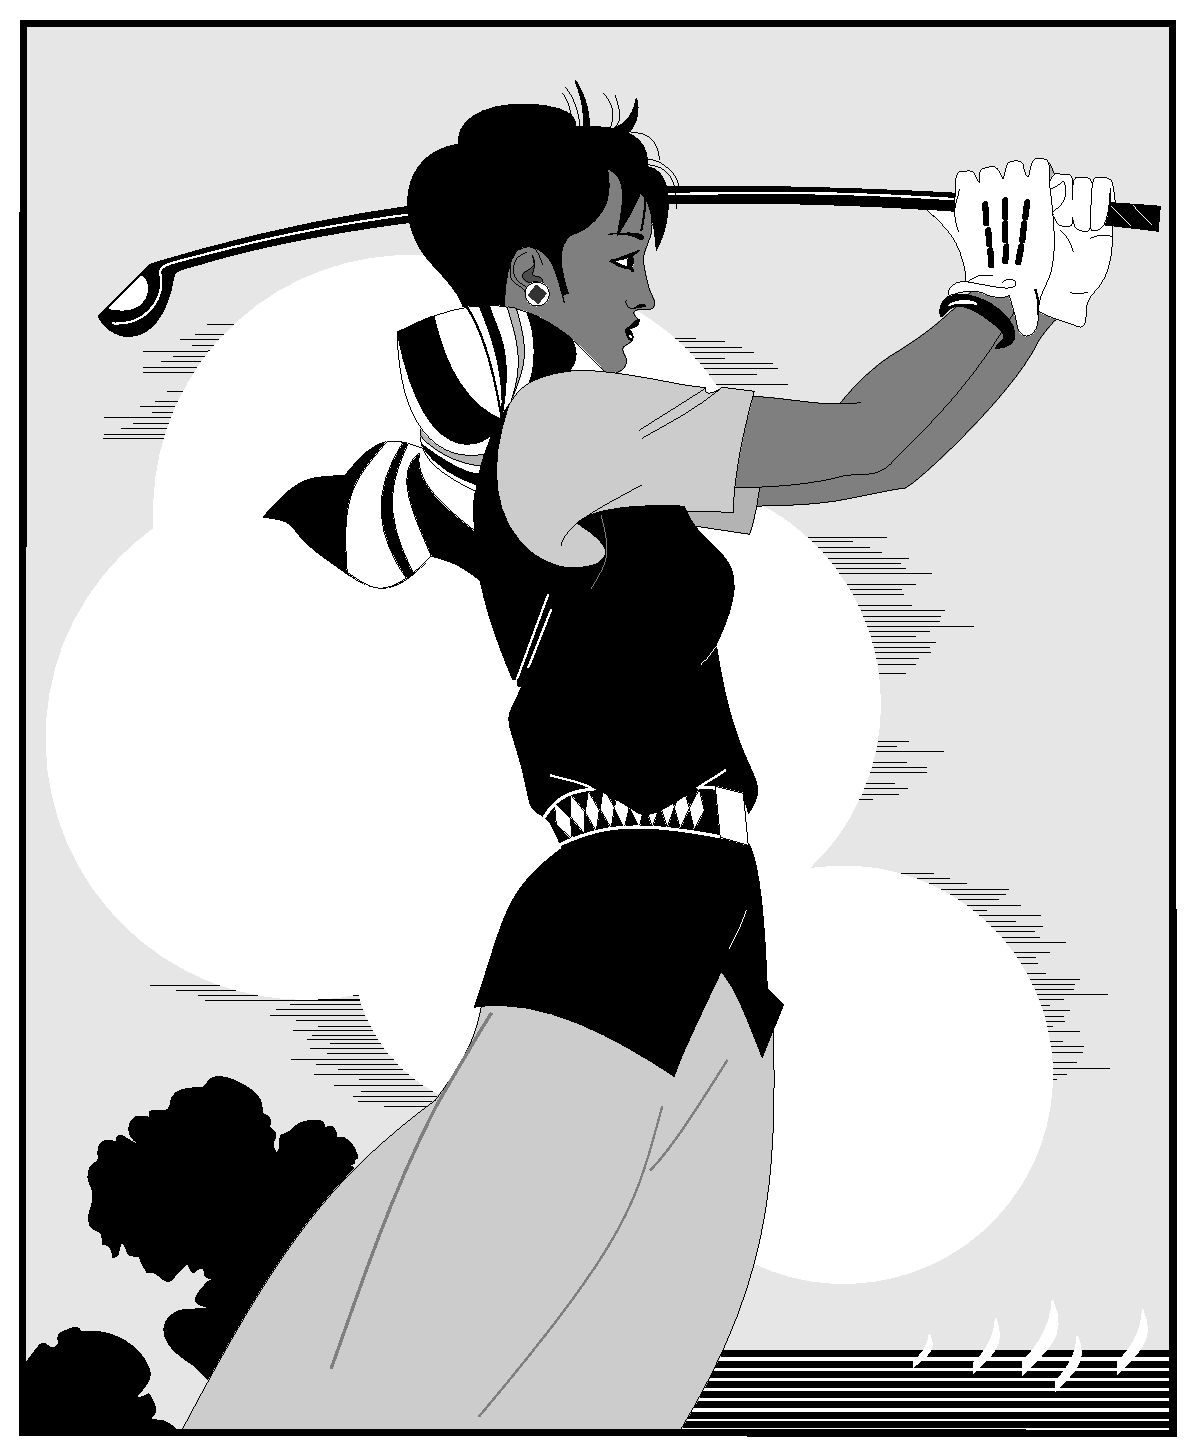
\includegraphics[width = 0.4\textwidth]{golfer}
\bicaption[golfer5]{}{打高尔夫球的人}{Fig.$\!$}{The person playing golf}\vspace{-1em}
\end{figure}

附录中公式的示例:
\begin{align}
a & = b \times c \\
E & = m c^2
\end{align}
